% Suggested time: 3-4 minutes (includes the live screen recording)
\section{Python Implementation and Results}

\begin{frame}{Code Components}
  \small
  \begin{tabularx}{\textwidth}{l >{\raggedright\arraybackslash}X}
    \toprule
    \textbf{Code} & \textbf{What it does} \\
    \midrule
    \texttt{data/*.csv} & Input: vertices (\texttt{locations.csv}) and weights (\texttt{distance\_matrix\_km.csv}) \\
    \texttt{split} & Divide: random axis, sort, median cut \\
    \texttt{solve} & Recursion and base cases; records each step \\
    \texttt{shortest\_bridge}, \texttt{merge} & Combine: bridge, remove 2 edges, add 2, smallest $\Delta$ \\
    \texttt{check\_route} & Valid closed tour? Recompute the total from the weights \\
    \texttt{held\_karp} & Exact optimum, \emph{for comparison only} \\
    \bottomrule
  \end{tabularx}
\end{frame}

\begin{frame}{Live Demo}
  \centering
  \Large\texttt{python main.py}
  \bigskip

  \normalsize
  \begin{enumerate}
    \item Input data: vertices and weight matrix
    \item Every divide, base-case and merge step, with its arithmetic
    \item Resulting route and total distance
    \item Verification checks
    \item Comparison with the exact optimum
  \end{enumerate}
  \bigskip
  \groupnote{Switch to the screen recording here}
\end{frame}

\begin{frame}{Resulting Route: \DCTotal{} km}
  \centering
  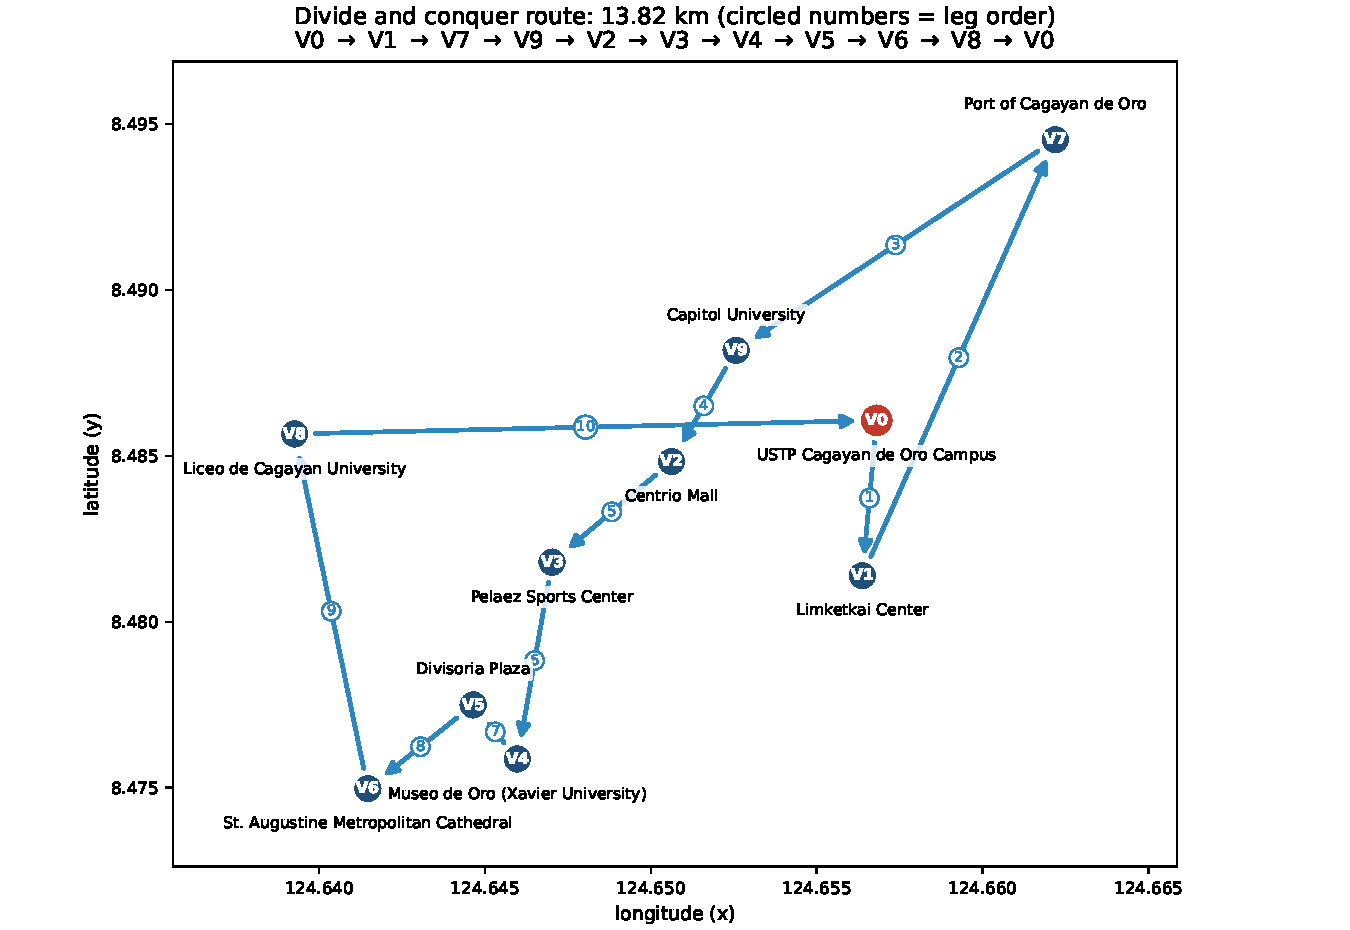
\includegraphics[height=0.86\textheight]{route.pdf}
\end{frame}

\begin{frame}{Verification: Recomputing the Total}
  \centering
  \scriptsize
  \setlength{\tabcolsep}{4pt}
  % AUTO-GENERATED by code/main.py --export-latex. Do not edit; re-run the export instead.
\begin{tabular}{c l l r r}
\toprule
\textbf{Leg} & \textbf{From} & \textbf{To} & \textbf{km} & \textbf{Cumulative} \\
\midrule
1 & V0 USTP Cagayan de Oro Campus & V1 Limketkai Center & 1.09 & 1.09 \\
2 & V1 Limketkai Center & V7 Port of Cagayan de Oro & 2.32 & 3.41 \\
3 & V7 Port of Cagayan de Oro & V9 Capitol University & 1.79 & 5.20 \\
4 & V9 Capitol University & V2 Centrio Mall & 0.58 & 5.78 \\
5 & V2 Centrio Mall & V3 Pelaez Sports Center & 1.18 & 6.96 \\
6 & V3 Pelaez Sports Center & V4 Museo de Oro (Xavier University) & 1.31 & 8.27 \\
7 & V4 Museo de Oro (Xavier University) & V5 Divisoria Plaza & 0.54 & 8.81 \\
8 & V5 Divisoria Plaza & V6 St. Augustine Metropolitan Cathedral & 0.74 & 9.55 \\
9 & V6 St. Augustine Metropolitan Cathedral & V8 Liceo de Cagayan University & 1.65 & 11.20 \\
10 & V8 Liceo de Cagayan University & V0 USTP Cagayan de Oro Campus & 2.62 & 13.82 \\
\midrule
\multicolumn{3}{r}{\textbf{Total}} & \multicolumn{2}{r}{\textbf{13.82 km}} \\
\bottomrule
\end{tabular}


  \medskip
  \footnotesize
  \textbf{Checks (all \DCAllChecks{}):} starts at V0 \textbullet{} returns to V0 \textbullet{}
  \NumVertices{} legs \textbullet{} each location exactly once \textbullet{}
  recomputed \DCRecomputed{} km = reported \DCTotal{} km
\end{frame}
